% To familiarize yourself with this template, the body contains
% some examples of its use.  Look them over.  Then you can
% run LaTeX on this file.  After you have LaTeXed this file then
% you can look over the result either by printing it out with
% dvips or using xdvi.
%

\documentclass[twoside]{article}
%\usepackage{soul}
\usepackage{./lecnotes_macros}


\begin{document}
%FILL IN THE RIGHT INFO.
%\lecture{**LECTURE-NUMBER**}{**DATE**}{**LECTURERS**}{**SCRIBE**}
\lecture{2}{19 January 2025}{Maria Francis and M. V. Panduranga Rao}{Gautam Singh}
%\footnotetext{These notes are partially based on those of Nigel Mansell.}

%All figures are to be placed in a separate folder named ``images''

% **** YOUR NOTES GO HERE:

\section{Cryptanalysis of DES Reduced to 4 Rounds}
The notation for this reduced DES cryptosystem is shown in \autoref{fig:des-4}.

\begin{figure}[!ht]
    \centering
    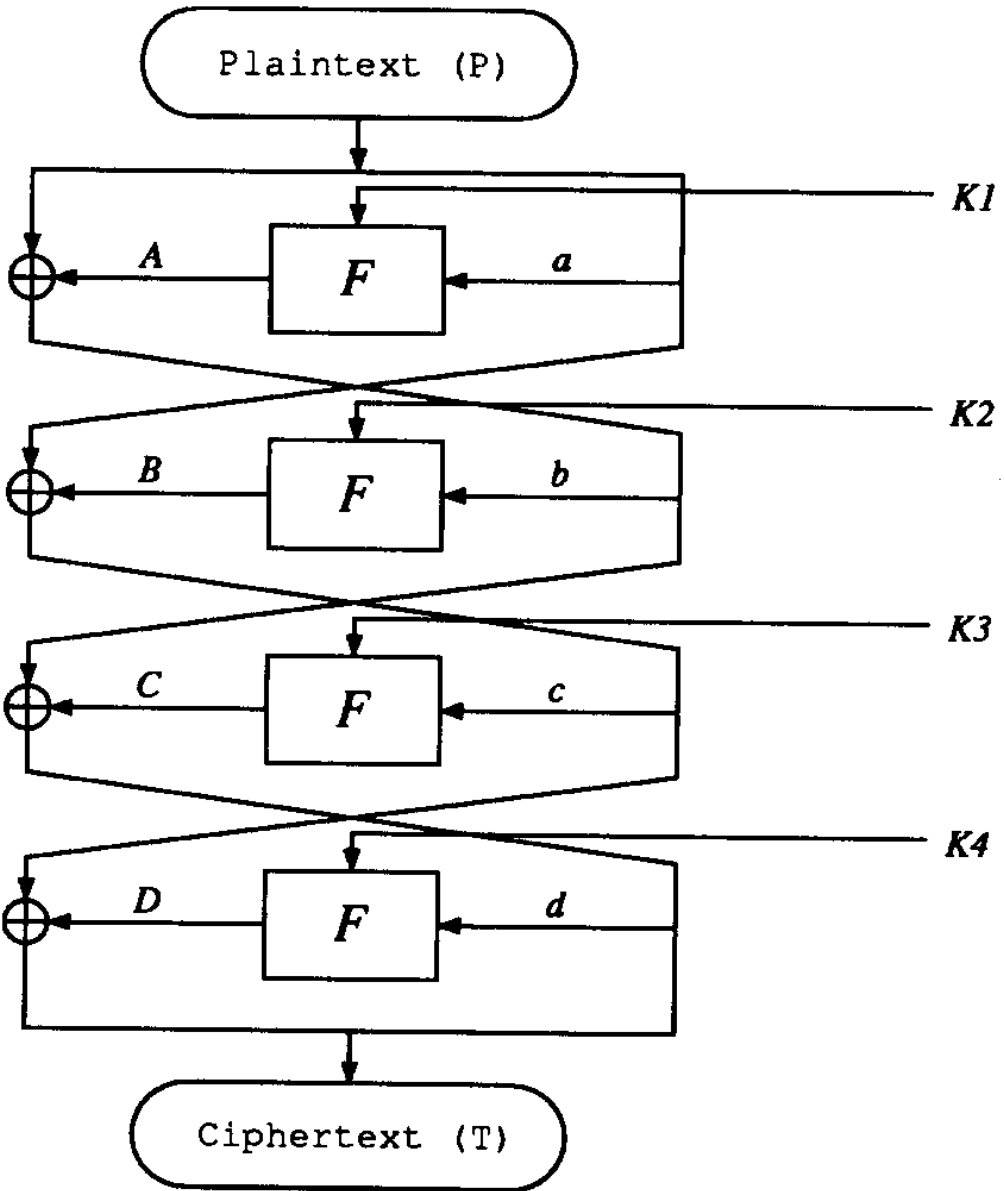
\includegraphics[width=0.5\linewidth]{images/des_4round.png}
    \caption{DES reduced to four rounds.}
    \label{fig:des-4}
\end{figure}

To find the master key, we make use of the characteristic shown in
\autoref{fig:des-4-char}. Using this characteristic, we have \(a^\prime = 0_x
\implies A^\prime = 0_x\). Thus, \(b = \texttt{20 00 00 00}\) necessarily, and
the single bit difference only diffuses from here on.

Since \(a^\prime = 0\), we write
\begin{align}
    c^\prime &= D^\prime \oplus l^\prime = a^\prime \oplus B^\prime \\
    \implies D^\prime &= l^\prime \oplus B^\prime,
    \label{eq:des-4rd-D}
\end{align}

where \(T^\prime = \brak{l^\prime, r^\prime}\) is the ciphertext XOR. Further,
we have \(d^\prime = r^\prime\), so \(d^\prime\) is completely known. Observe
that \(S^\prime_{Eb} = 0\) for S2, \dots, S8. Thus, \(S^\prime_{Ob} = 0\) always
for 28 bits. Hence, \(S^\prime_{Od}\) is known for S2, \dots, S8. We find the
6-bit subkey blocks corresponding \(S_{Kd}\) using bruteforce to verify
\eqref{eq:des-4rd-k4}. 

\begin{equation}
    S\brak{S_{Ed} \oplus S_{Kd}} \oplus S\brak{S^*_{Ed} \oplus S_{Kd}} = S^\prime_{Od}.
    \label{eq:des-4rd-k4}
\end{equation}

Since \(\Omega_P^1\) has probability 1 and \(\brak{d^\prime, D^\prime}\) is a
right pair, we will find the right value of \(S_{Kd}\) with probability 1. Thus,
we have found 42 bits of the subkey \(K4\). If the DES key-scheduling algorithm
is followed, these correspond to 42 key bits of the master key \(K\). Finding
the other 14 bits can be done by exhaustively searching the \(2^{14}\)
possibilities and verifying that the plaintexts are correctly encrypted. This
leads to an attack with \(2^{14}\) encryptions, which runs efficiently.

\begin{figure}[!ht]
    \centering
    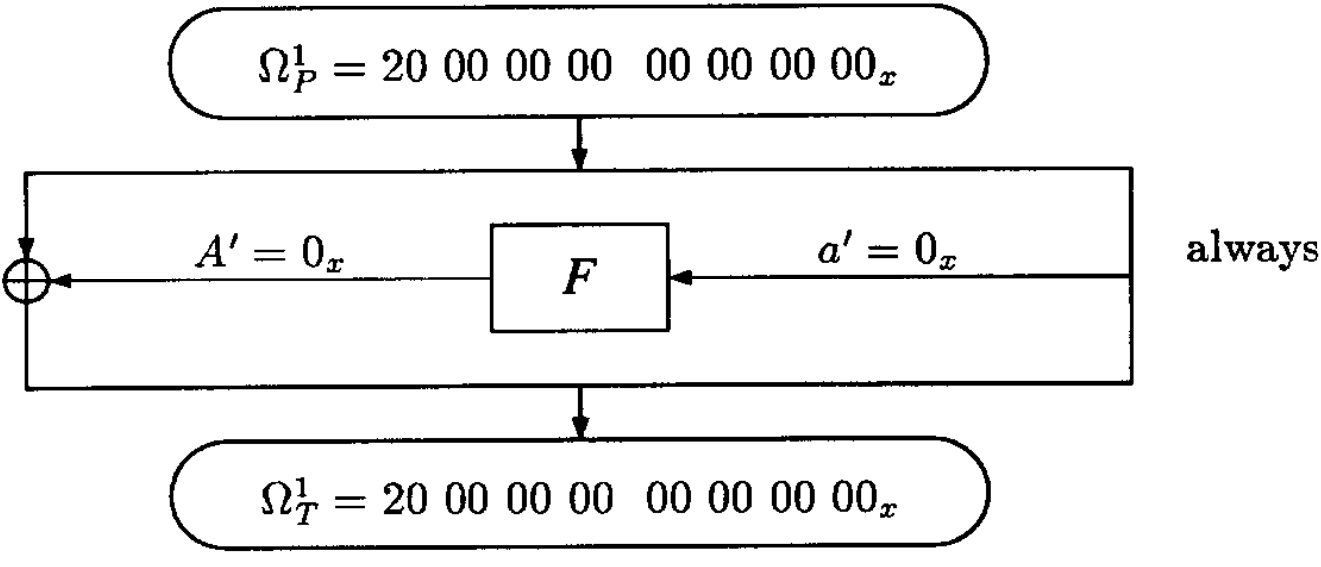
\includegraphics[width=0.5\linewidth]{images/des_4round_char.png}
    \caption{Characteristic used for cryptanalysis of DES reduced to four rounds.}
    \label{fig:des-4-char}
\end{figure}

\subsection{DES With Independent Subkeys}

Differential cryptanalysis can also work if the subkeys \(K1,\ldots,K4\) are
generated independently and do not depend on a key-scheduling algorithm. As
before, we can find 42 bits of \(K4\). To find the remaining 6 bits, we use
\(\Omega_P^2\) shown in \autoref{fig:des-4-char-2}. With this characteristic, we
have \(S1^\prime_{Eb} = 0\), thus using a similar argument we can find
\(S1^\prime_{Od}\) and apply the counting approach to get \(S1_{Kd}\), which
will completely find \(K4\).

\begin{figure}[!ht]
    \centering
    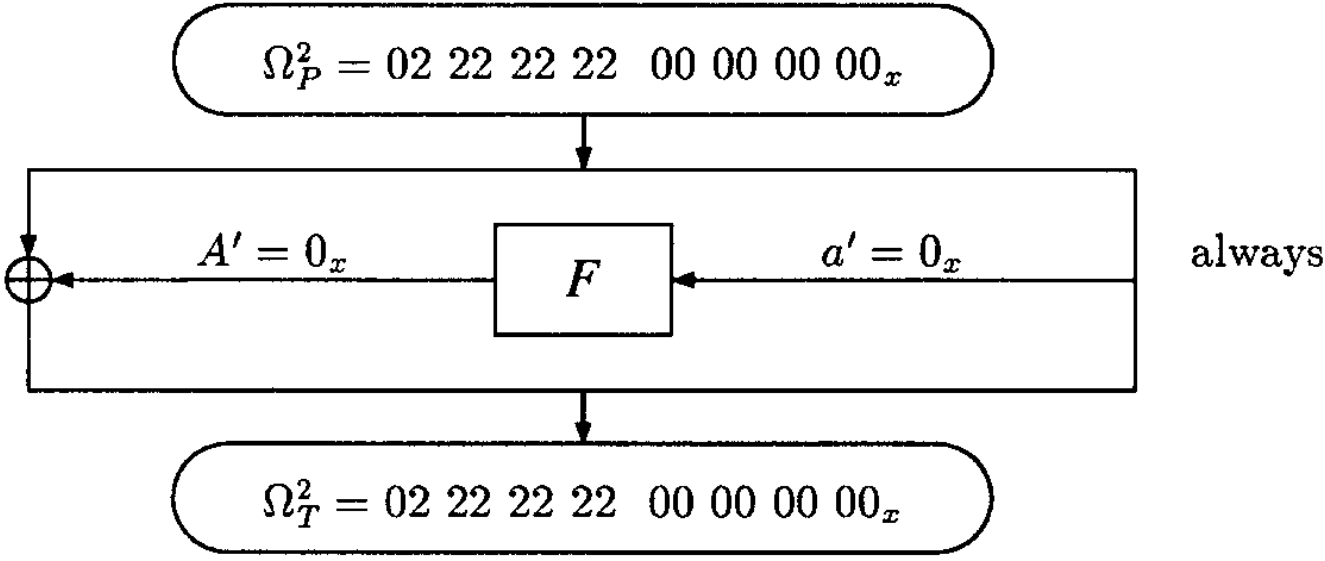
\includegraphics[width=0.5\linewidth]{images/des_4round_char2.png}
    \caption{Second characteristic used to find K3 and K4 completely.}
    \label{fig:des-4-char-2}
\end{figure}

Finding \(K3\) using \(\Omega_P^2\) is straightforward. At this point, we can
decrypt the fourth round to completely find \(c^\prime\) and \(C^\prime =
b^\prime \oplus D^\prime\). A similar counting argument can be used to find
\(K3\) completely.

To find \(K1\) and \(K2\) we will need to choose different characteristics,
since both characteristics have \(a^\prime = 0 \rightarrow A^\prime = 0\) and
thus all keys are equally likely for \(K1\). Similarly, some \(S\) boxes in the
second round have zero XOR inputs and make all keys equally likely. To overcome
these, we choose characteristics \(\Omega_P^3\) and \(\Omega_P^4\) arbitrarily
such that
\begin{enumerate}
    \item \(S^\prime_{Ea} \neq 0\) for all S boxes for both characteristics.
    \item For every S box the \(S^\prime_{Ea}\) values differ between the
    characteristics.
\end{enumerate}

Knowing the value of \(b^\prime\) after decryption of the third round, we can
find \(B^\prime = c^\prime \oplus a^\prime = c^\prime \oplus R^\prime\). A
similar counting argument will find the complete \(K2\). Similarly, \(A^\prime =
L^\prime \oplus b^\prime\) and thus the complete \(K1\) can also be found. One
can verify the keys have been found by encrypting plaintexts with these values
and checking the outputs. This completes the cryptanalysis of DES reduced to 4
rounds. It also shows that differential cryptanalysis can work even if the round
subkeys in DES are independently chosen.

For the cryptanalysis, a total of 16 encryptions are needed to find the keys
with high probability: 8 pairs each of \(\Omega^1\) and \(\Omega^2\) and 4 pairs
each of \(\Omega^3\) and \(\Omega^4\).

\section{DES Reduced to 6 Rounds}

For the cryptanalysis of DES reduced to 6 rounds, we make use of two
characteristics, both with probability \(\frac{1}{16}\) as shown in
\autoref{fig:des-6-char}.

\begin{figure}[!ht]
    \centering
    \begin{subfigure}{0.45\linewidth}
        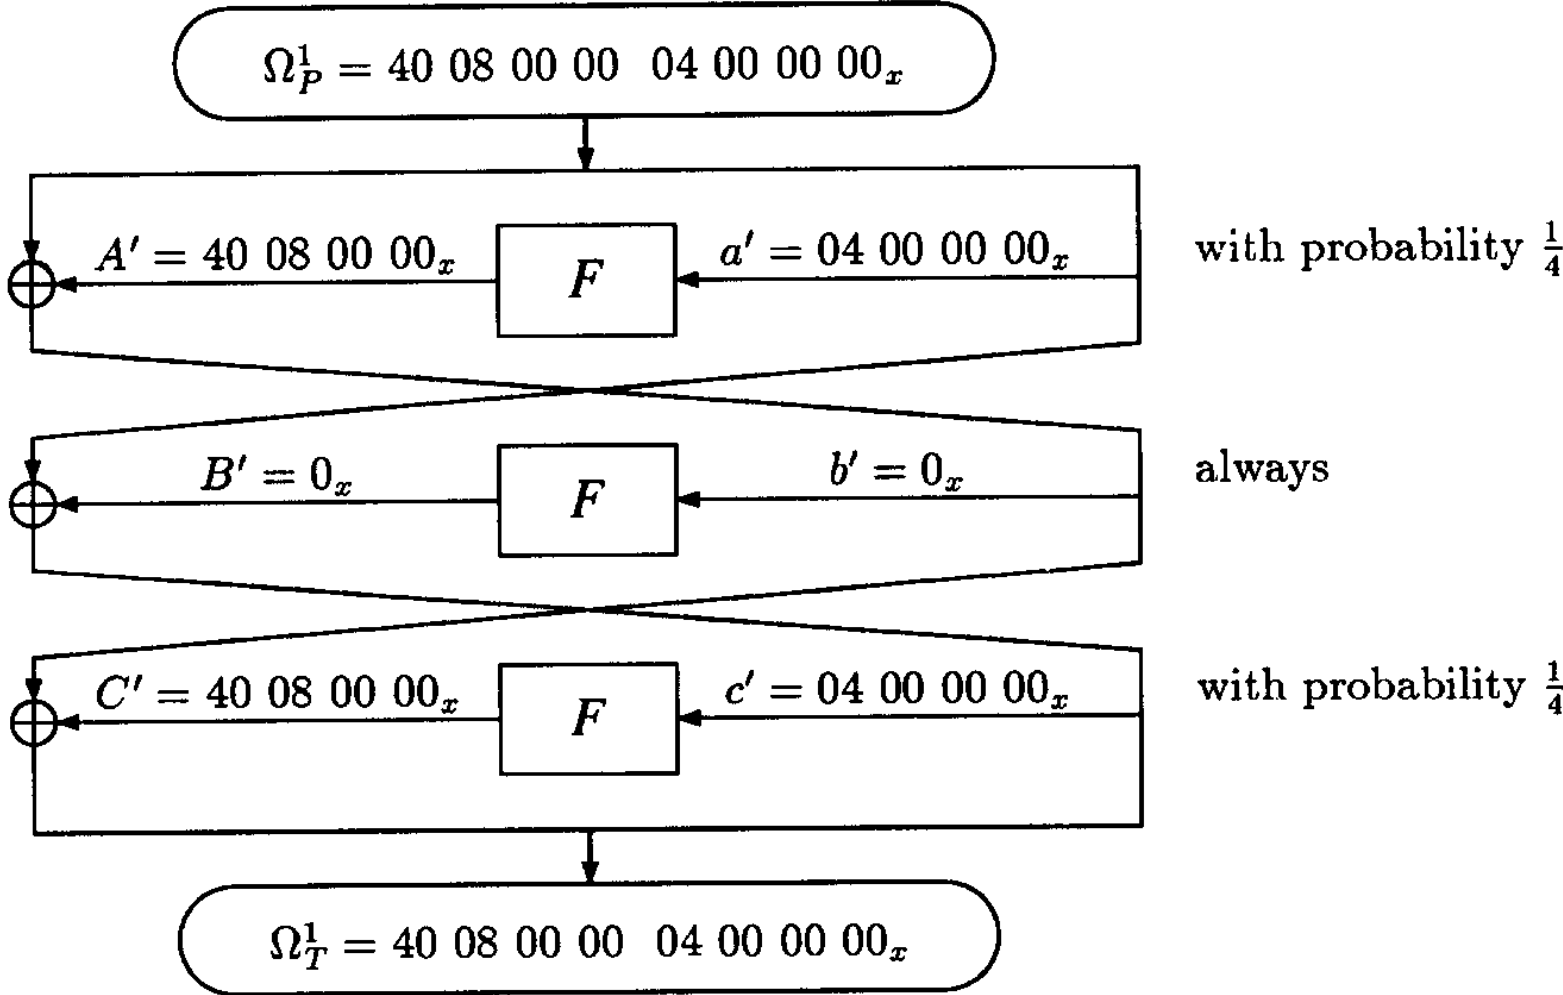
\includegraphics[width=\linewidth]{images/des_6round_char1.png}
        \label{fig:des-6-char1}
    \end{subfigure}
    \hfill
    \begin{subfigure}{0.45\linewidth}
        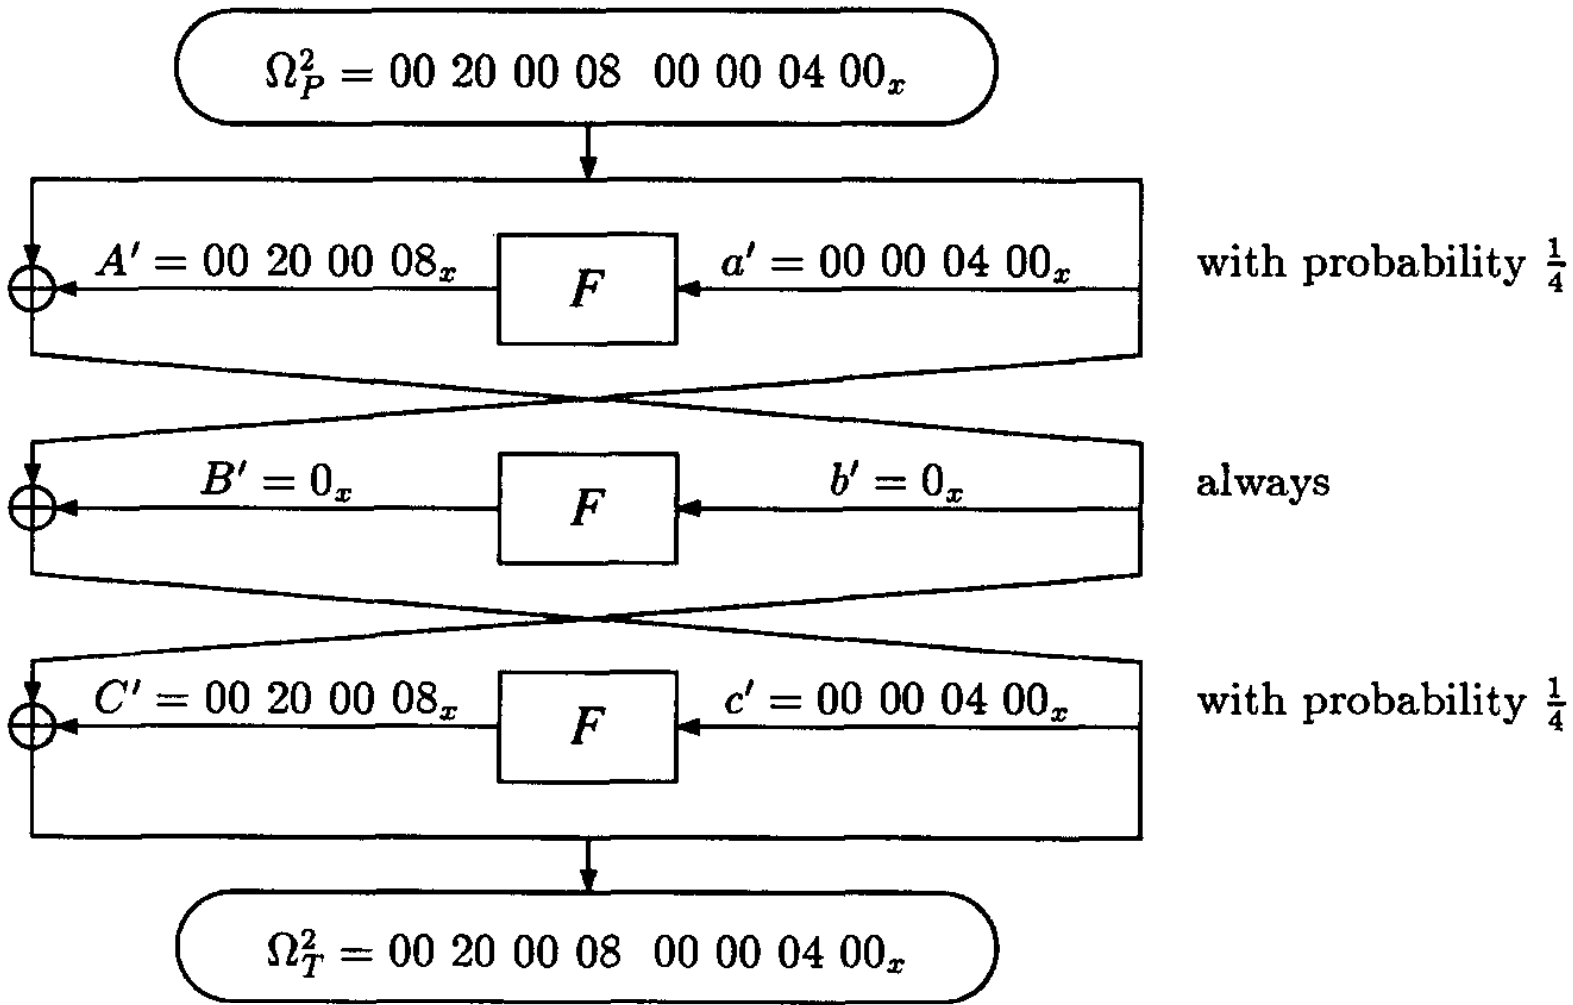
\includegraphics[width=\linewidth]{images/des_6round_char2.png}
        \label{fig:des-6-char2}
    \end{subfigure}
    \caption{Characteristics used for cryptanalysis of DES reduced to 6 rounds.}
    \label{fig:des-6-char}
\end{figure}

For the characteristic \(\Omega_P^1\), the S boxes S2, S5, \dots, S8 have zero
input XORs and for \(\Omega_P^2\), the S boxes S1, S2, S4, S5 and S6 have zero
input XORs in the fourth round. Note that \(d^\prime = b^\prime \oplus C^\prime
= C^\prime\). We write

\end{document}
